% =====================================================================
%  MSACL DS301 Deep Learning · Quiz 1 · Foundations
%  Academic problem-set style (single-source, \ifsolution toggle)
%  SINGLE SOURCE — produces BOTH the student quiz and the answer key.
%
%  ANSWER TOGGLE
%  -------------
%  Student version (answers HIDDEN) — the default:
%       pdflatex quiz01_foundations.tex
%  Answer key (answers SHOWN):
%       pdflatex "\def\showsolutions{}% =====================================================================
%  MSACL DS301 Deep Learning · Quiz 1 · Foundations
%  Academic problem-set style (single-source, \ifsolution toggle)
%  SINGLE SOURCE — produces BOTH the student quiz and the answer key.
%
%  ANSWER TOGGLE
%  -------------
%  Student version (answers HIDDEN) — the default:
%       pdflatex quiz01_foundations.tex
%  Answer key (answers SHOWN):
%       pdflatex "\def\showsolutions{}% =====================================================================
%  MSACL DS301 Deep Learning · Quiz 1 · Foundations
%  Academic problem-set style (single-source, \ifsolution toggle)
%  SINGLE SOURCE — produces BOTH the student quiz and the answer key.
%
%  ANSWER TOGGLE
%  -------------
%  Student version (answers HIDDEN) — the default:
%       pdflatex quiz01_foundations.tex
%  Answer key (answers SHOWN):
%       pdflatex "\def\showsolutions{}% =====================================================================
%  MSACL DS301 Deep Learning · Quiz 1 · Foundations
%  Academic problem-set style (single-source, \ifsolution toggle)
%  SINGLE SOURCE — produces BOTH the student quiz and the answer key.
%
%  ANSWER TOGGLE
%  -------------
%  Student version (answers HIDDEN) — the default:
%       pdflatex quiz01_foundations.tex
%  Answer key (answers SHOWN):
%       pdflatex "\def\showsolutions{}\input{quiz01_foundations.tex}"
%  (or, to flip by hand, change \solutionfalse to \solutiontrue below.)
% =====================================================================
\documentclass[11pt]{article}

\newif\ifsolution
\ifdefined\showsolutions \solutiontrue \else \solutionfalse \fi
% \solutiontrue   % <-- uncomment to hard-code the ANSWER KEY build

\usepackage[letterpaper, margin=0.6in, top=0.7in, bottom=0.5in]{geometry}
\usepackage{amsmath, amssymb}
\usepackage{xcolor}
\usepackage{tikz}
\usepackage{fancyhdr}

\pagestyle{fancy}
\fancyhf{}
\fancyhead[L]{\small\textbf{MSACL DS301 --- Deep Learning}}
\fancyhead[R]{\small\textbf{Quiz 1: Foundations\ifsolution\ \textmd{(Answer Key)}\fi}}
\fancyfoot[C]{\thepage}
\renewcommand{\headrulewidth}{0.4pt}

\newcommand{\blk}[1]{\underline{\hspace{#1}}}
% Reveal-or-blank: shows the answer in the key, a blank rule on the student sheet.
\newcommand{\rb}[2]{\ifsolution\textbf{#1}\else\blk{#2}\fi}
% Boxed answer (key only) and blank writing space (student only).
\newcommand{\keybox}[1]{\ifsolution\par\vspace{2pt}%
  \fbox{\parbox{0.965\textwidth}{\small\textbf{Answer.}\; #1}}\par\fi}
\newcommand{\work}[1]{\ifsolution\else\vspace{#1}\fi}

\setlength{\parindent}{0pt}
\setlength{\parskip}{3pt}
\setlength{\abovedisplayskip}{5pt}
\setlength{\belowdisplayskip}{5pt}

\begin{document}

\begin{center}
{\Large \textbf{Quiz 1 --- Foundations}}\\[2pt]
{\normalsize The neuron, activation functions, a layer as a matrix, and a two-layer pass}
\end{center}

\vspace{-2pt}
\begin{center}
\fbox{\parbox{0.92\textwidth}{\small
\textbf{Instructions:}\; Answer all six questions. Intuition first, light arithmetic ---
show your work on the blanks. No calculators needed.%
\ifsolution\else\\[4pt]\textbf{Name:}\ \blk{6cm}\hfill\textbf{Date:}\ \blk{3.5cm}\fi
}}
\end{center}

\vspace{-2pt}\hrule\vspace{5pt}

% =========================== Q1 ===========================
\textbf{1. Pick the activation, then compute.}\; {\small Your MRSA classifier's \emph{final} neuron
must output a probability between $0$ and $1$ that the isolate is \emph{resistant}. The three
activation shapes are below.}

\vspace{3pt}
\begin{center}
\newcommand{\axes}{\draw[->,gray] (-1.6,0)--(1.95,0); \draw[->,gray] (0,-0.9)--(0,1.6);}
%
\begin{minipage}[t]{0.31\linewidth}\centering

\begin{tikzpicture}[scale=0.9, line cap=round]
  \axes
  \draw[very thick, samples=80, domain=-1.5:1.85] plot (\x,{1.2/(1+exp(-4*\x))});
\end{tikzpicture}\\[2pt]
(a) Sigmoid
\end{minipage}\hfill
%
\begin{minipage}[t]{0.31\linewidth}\centering
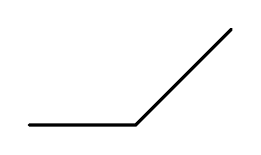
\begin{tikzpicture}[scale=0.9, line cap=round]
  \axes
  \draw[very thick] (-1.5,0)--(0,0)--(1.35,1.35);
\end{tikzpicture}\\[2pt]
(b) ReLU
\end{minipage}\hfill
%
\begin{minipage}[t]{0.31\linewidth}\centering

\begin{tikzpicture}[scale=0.9, line cap=round]
  \axes
  \draw[very thick] (-1.4,-0.8)--(1.4,1.3);
\end{tikzpicture}\\[2pt]
(c) Linear
\end{minipage}
\end{center}

\vspace{4pt}
{\small (i) Which curve --- (a), (b), or (c) --- belongs on that final neuron, and why?}\\[2pt]
\hspace*{1.5em}\rb{(a) Sigmoid --- its output is squeezed into $(0,1)$, so it reads as a probability}{10.5cm}\\[6pt]
{\small (ii) A hidden \textbf{ReLU} neuron receives weighted sum $z=-3$. Its output $=$}\;\; \rb{$0$}{1.6cm}\\[6pt]
{\small (iii) The final \textbf{sigmoid} neuron receives $z=0$. The probability it reports $\approx$}\;\; \rb{$0.5$}{1.6cm}

\keybox{(i) Curve \textbf{(a), the sigmoid} --- it is the only activation whose output is bounded
to $(0,1)$, so it can be read as a probability; ReLU is unbounded above and the linear line is
unbounded both ways, so neither can report a probability. (ii) $\operatorname{ReLU}(-3)=\max(0,-3)=0$
--- the neuron is silent. (iii) $\operatorname{sigmoid}(0)=1/(1+e^{0})=1/2=0.5$ --- maximally
uncertain, a coin flip.}

\vspace{2pt}\hrule\vspace{5pt}

% =========================== Q2 ===========================
\textbf{2. One neuron, by hand.}\; {\small Compute the weighted sum $z$, then pass it through
ReLU.}

\vspace{2pt}
\textbf{Given:}\quad $x_1 = 2,\ \ x_2 = 3 \qquad w_1 = 0.5,\ \ w_2 = -1 \qquad b = 1$

\[
z = w_1 x_1 + w_2 x_2 + b = \blk{5.5cm} = \rb{$-1$}{1.3cm}
\]
\[
\text{output} = \operatorname{ReLU}(z) = \max(0,\,z) = \rb{$0$}{1.3cm}
\]

\work{0.9cm}

\keybox{$z = (0.5)(2) + (-1)(3) + 1 = 1 - 3 + 1 = -1$, so
$\operatorname{ReLU}(-1) = \max(0,-1) = 0$. ReLU clips the negative sum to zero: for this
input the neuron stays silent.}

\vspace{2pt}\hrule\vspace{5pt}

% =========================== Q3 ===========================
\textbf{3. A whole layer in one step.}\; {\small Multiply the $2\times3$ weight matrix by the
input vector.}

\[
\mathbf{W}\mathbf{x} =
\underbrace{\begin{pmatrix} 1 & 0 & 2 \\ -1 & 3 & 1 \end{pmatrix}}_{\mathbf{W}}
\underbrace{\begin{pmatrix} 2 \\ 1 \\ 0 \end{pmatrix}}_{\mathbf{x}}
= \begin{pmatrix} \blk{3.4cm} \\[3pt] \blk{3.4cm} \end{pmatrix}
= \begin{pmatrix} \rb{$2$}{1cm} \\[3pt] \rb{$1$}{1cm} \end{pmatrix}
\]

\work{0.7cm}

\keybox{Row 1: $(1)(2)+(0)(1)+(2)(0) = 2$. \ Row 2: $(-1)(2)+(3)(1)+(1)(0) = 1$. \ Hence
$\mathbf{W}\mathbf{x} = \left(\begin{smallmatrix}2\\1\end{smallmatrix}\right)$. A $2\times3$
matrix times a length-$3$ vector yields a length-$2$ output --- one number per neuron: a full
forward pass.}

\vspace{2pt}\hrule\vspace{5pt}

% =========================== Q4 ===========================
\textbf{4. Learned or engineered?}\; {\small Two ways to call \emph{resistant} vs.\
\emph{susceptible} from a MALDI-TOF spectrum:}

\vspace{2pt}
\textbf{Pipeline A} --- a technician computes the peak area at $m/z\ 2415$ and the $2415/4100$
ratio, then feeds those two numbers to logistic regression.

\textbf{Pipeline B} --- the raw $6{,}000$-bin spectrum goes straight into a neural network,
which forms its own internal ``peak-ish here'' detector in an early layer.

\vspace{3pt}
Which pipeline uses \emph{hand-engineered} features, and which uses \emph{learned} features?

\vspace{3pt}
hand-engineered $\rightarrow$ Pipeline \rb{A}{1.6cm}
\hfill
learned $\rightarrow$ Pipeline \rb{B}{1.6cm}
\hspace*{2cm}

\keybox{Hand-engineered $\rightarrow$ A; learned $\rightarrow$ B. In A a human chose the peak
area and the ratio (hand-engineered features); in B the network discovers its own ``peak-ish''
detector directly from the raw spectrum (learned features). That shift is the essence of deep
learning.}

\vspace{2pt}\hrule\vspace{5pt}

% =========================== Q5 ===========================
\textbf{5. In one sentence.}\; {\small What is the core difference between deep learning and
classic machine learning?}

\work{1.4cm}
\ifsolution\else\blk{\linewidth}\\[10pt]\blk{\linewidth}\fi

\keybox{Deep learning learns its own features straight from raw data, whereas classic machine
learning relies on features a human engineers first. (Any answer capturing ``learned features
from raw data'' vs.\ ``human-engineered features'' earns full credit; phrasing about
representation learning or end-to-end training is equally acceptable.)}

\vspace{2pt}\hrule\vspace{5pt}

% =========================== Q6 ===========================
\textbf{6. Two layers, by hand.}\; {\small Run a full two-layer forward pass: first the
hidden layer (matrix--vector, add bias, then ReLU), then the output layer.}

\vspace{2pt}
\textbf{Layer 1:}\quad
$\mathbf{W_1} = \begin{pmatrix} 1 & -1 \\ -1 & 1 \end{pmatrix},\quad
\mathbf{x} = \begin{pmatrix} 2 \\ 1 \end{pmatrix},\quad
\mathbf{b_1} = \begin{pmatrix} 0 \\ -4 \end{pmatrix}$

\[
\mathbf{h} = \operatorname{ReLU}(\mathbf{W_1}\mathbf{x} + \mathbf{b_1})
= \operatorname{ReLU}\!\begin{pmatrix} \blk{2.2cm} \\[3pt] \blk{2.2cm} \end{pmatrix}
= \begin{pmatrix} \rb{$1$}{1cm} \\[3pt] \rb{$0$}{1cm} \end{pmatrix}
\]

\textbf{Layer 2:}\quad
$\mathbf{W_2} = \begin{pmatrix} 3 & 2 \end{pmatrix},\quad b_2 = -1$

\[
y = \mathbf{W_2}\mathbf{h} + b_2 = \blk{5cm} = \rb{$2$}{1.3cm}
\]

\work{0.9cm}

\keybox{Layer 1: row 1 $=(1)(2)+(-1)(1)+0 = 1$, so $\operatorname{ReLU}(1)=1$; row 2
$=(-1)(2)+(1)(1)+(-4) = -5$, so $\operatorname{ReLU}(-5)=0$. Hence
$\mathbf{h} = \left(\begin{smallmatrix}1\\0\end{smallmatrix}\right)$ --- the second hidden
neuron stays silent. Layer 2: $y = (3)(1)+(2)(0)-1 = 2$. The input $(2,1)$ here is the
layer output $\mathbf{Wx}$ from Q3 carried forward --- a layer's output is simply the
next layer's input, and stacking that same move is what ``deep'' means.}

\vspace{4pt}\hrule\vspace{3pt}
{\small\itshape \ifsolution Answer key.\else Keep this sheet --- the neuron and matrix drills
are your Lab 1 cheat-sheet.\fi}

\end{document}
"
%  (or, to flip by hand, change \solutionfalse to \solutiontrue below.)
% =====================================================================
\documentclass[11pt]{article}

\newif\ifsolution
\ifdefined\showsolutions \solutiontrue \else \solutionfalse \fi
% \solutiontrue   % <-- uncomment to hard-code the ANSWER KEY build

\usepackage[letterpaper, margin=0.6in, top=0.7in, bottom=0.5in]{geometry}
\usepackage{amsmath, amssymb}
\usepackage{xcolor}
\usepackage{tikz}
\usepackage{fancyhdr}

\pagestyle{fancy}
\fancyhf{}
\fancyhead[L]{\small\textbf{MSACL DS301 --- Deep Learning}}
\fancyhead[R]{\small\textbf{Quiz 1: Foundations\ifsolution\ \textmd{(Answer Key)}\fi}}
\fancyfoot[C]{\thepage}
\renewcommand{\headrulewidth}{0.4pt}

\newcommand{\blk}[1]{\underline{\hspace{#1}}}
% Reveal-or-blank: shows the answer in the key, a blank rule on the student sheet.
\newcommand{\rb}[2]{\ifsolution\textbf{#1}\else\blk{#2}\fi}
% Boxed answer (key only) and blank writing space (student only).
\newcommand{\keybox}[1]{\ifsolution\par\vspace{2pt}%
  \fbox{\parbox{0.965\textwidth}{\small\textbf{Answer.}\; #1}}\par\fi}
\newcommand{\work}[1]{\ifsolution\else\vspace{#1}\fi}

\setlength{\parindent}{0pt}
\setlength{\parskip}{3pt}
\setlength{\abovedisplayskip}{5pt}
\setlength{\belowdisplayskip}{5pt}

\begin{document}

\begin{center}
{\Large \textbf{Quiz 1 --- Foundations}}\\[2pt]
{\normalsize The neuron, activation functions, a layer as a matrix, and a two-layer pass}
\end{center}

\vspace{-2pt}
\begin{center}
\fbox{\parbox{0.92\textwidth}{\small
\textbf{Instructions:}\; Answer all six questions. Intuition first, light arithmetic ---
show your work on the blanks. No calculators needed.%
\ifsolution\else\\[4pt]\textbf{Name:}\ \blk{6cm}\hfill\textbf{Date:}\ \blk{3.5cm}\fi
}}
\end{center}

\vspace{-2pt}\hrule\vspace{5pt}

% =========================== Q1 ===========================
\textbf{1. Pick the activation, then compute.}\; {\small Your MRSA classifier's \emph{final} neuron
must output a probability between $0$ and $1$ that the isolate is \emph{resistant}. The three
activation shapes are below.}

\vspace{3pt}
\begin{center}
\newcommand{\axes}{\draw[->,gray] (-1.6,0)--(1.95,0); \draw[->,gray] (0,-0.9)--(0,1.6);}
%
\begin{minipage}[t]{0.31\linewidth}\centering

\begin{tikzpicture}[scale=0.9, line cap=round]
  \axes
  \draw[very thick, samples=80, domain=-1.5:1.85] plot (\x,{1.2/(1+exp(-4*\x))});
\end{tikzpicture}\\[2pt]
(a) Sigmoid
\end{minipage}\hfill
%
\begin{minipage}[t]{0.31\linewidth}\centering
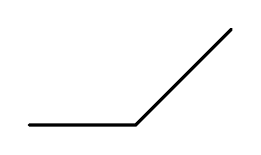
\begin{tikzpicture}[scale=0.9, line cap=round]
  \axes
  \draw[very thick] (-1.5,0)--(0,0)--(1.35,1.35);
\end{tikzpicture}\\[2pt]
(b) ReLU
\end{minipage}\hfill
%
\begin{minipage}[t]{0.31\linewidth}\centering

\begin{tikzpicture}[scale=0.9, line cap=round]
  \axes
  \draw[very thick] (-1.4,-0.8)--(1.4,1.3);
\end{tikzpicture}\\[2pt]
(c) Linear
\end{minipage}
\end{center}

\vspace{4pt}
{\small (i) Which curve --- (a), (b), or (c) --- belongs on that final neuron, and why?}\\[2pt]
\hspace*{1.5em}\rb{(a) Sigmoid --- its output is squeezed into $(0,1)$, so it reads as a probability}{10.5cm}\\[6pt]
{\small (ii) A hidden \textbf{ReLU} neuron receives weighted sum $z=-3$. Its output $=$}\;\; \rb{$0$}{1.6cm}\\[6pt]
{\small (iii) The final \textbf{sigmoid} neuron receives $z=0$. The probability it reports $\approx$}\;\; \rb{$0.5$}{1.6cm}

\keybox{(i) Curve \textbf{(a), the sigmoid} --- it is the only activation whose output is bounded
to $(0,1)$, so it can be read as a probability; ReLU is unbounded above and the linear line is
unbounded both ways, so neither can report a probability. (ii) $\operatorname{ReLU}(-3)=\max(0,-3)=0$
--- the neuron is silent. (iii) $\operatorname{sigmoid}(0)=1/(1+e^{0})=1/2=0.5$ --- maximally
uncertain, a coin flip.}

\vspace{2pt}\hrule\vspace{5pt}

% =========================== Q2 ===========================
\textbf{2. One neuron, by hand.}\; {\small Compute the weighted sum $z$, then pass it through
ReLU.}

\vspace{2pt}
\textbf{Given:}\quad $x_1 = 2,\ \ x_2 = 3 \qquad w_1 = 0.5,\ \ w_2 = -1 \qquad b = 1$

\[
z = w_1 x_1 + w_2 x_2 + b = \blk{5.5cm} = \rb{$-1$}{1.3cm}
\]
\[
\text{output} = \operatorname{ReLU}(z) = \max(0,\,z) = \rb{$0$}{1.3cm}
\]

\work{0.9cm}

\keybox{$z = (0.5)(2) + (-1)(3) + 1 = 1 - 3 + 1 = -1$, so
$\operatorname{ReLU}(-1) = \max(0,-1) = 0$. ReLU clips the negative sum to zero: for this
input the neuron stays silent.}

\vspace{2pt}\hrule\vspace{5pt}

% =========================== Q3 ===========================
\textbf{3. A whole layer in one step.}\; {\small Multiply the $2\times3$ weight matrix by the
input vector.}

\[
\mathbf{W}\mathbf{x} =
\underbrace{\begin{pmatrix} 1 & 0 & 2 \\ -1 & 3 & 1 \end{pmatrix}}_{\mathbf{W}}
\underbrace{\begin{pmatrix} 2 \\ 1 \\ 0 \end{pmatrix}}_{\mathbf{x}}
= \begin{pmatrix} \blk{3.4cm} \\[3pt] \blk{3.4cm} \end{pmatrix}
= \begin{pmatrix} \rb{$2$}{1cm} \\[3pt] \rb{$1$}{1cm} \end{pmatrix}
\]

\work{0.7cm}

\keybox{Row 1: $(1)(2)+(0)(1)+(2)(0) = 2$. \ Row 2: $(-1)(2)+(3)(1)+(1)(0) = 1$. \ Hence
$\mathbf{W}\mathbf{x} = \left(\begin{smallmatrix}2\\1\end{smallmatrix}\right)$. A $2\times3$
matrix times a length-$3$ vector yields a length-$2$ output --- one number per neuron: a full
forward pass.}

\vspace{2pt}\hrule\vspace{5pt}

% =========================== Q4 ===========================
\textbf{4. Learned or engineered?}\; {\small Two ways to call \emph{resistant} vs.\
\emph{susceptible} from a MALDI-TOF spectrum:}

\vspace{2pt}
\textbf{Pipeline A} --- a technician computes the peak area at $m/z\ 2415$ and the $2415/4100$
ratio, then feeds those two numbers to logistic regression.

\textbf{Pipeline B} --- the raw $6{,}000$-bin spectrum goes straight into a neural network,
which forms its own internal ``peak-ish here'' detector in an early layer.

\vspace{3pt}
Which pipeline uses \emph{hand-engineered} features, and which uses \emph{learned} features?

\vspace{3pt}
hand-engineered $\rightarrow$ Pipeline \rb{A}{1.6cm}
\hfill
learned $\rightarrow$ Pipeline \rb{B}{1.6cm}
\hspace*{2cm}

\keybox{Hand-engineered $\rightarrow$ A; learned $\rightarrow$ B. In A a human chose the peak
area and the ratio (hand-engineered features); in B the network discovers its own ``peak-ish''
detector directly from the raw spectrum (learned features). That shift is the essence of deep
learning.}

\vspace{2pt}\hrule\vspace{5pt}

% =========================== Q5 ===========================
\textbf{5. In one sentence.}\; {\small What is the core difference between deep learning and
classic machine learning?}

\work{1.4cm}
\ifsolution\else\blk{\linewidth}\\[10pt]\blk{\linewidth}\fi

\keybox{Deep learning learns its own features straight from raw data, whereas classic machine
learning relies on features a human engineers first. (Any answer capturing ``learned features
from raw data'' vs.\ ``human-engineered features'' earns full credit; phrasing about
representation learning or end-to-end training is equally acceptable.)}

\vspace{2pt}\hrule\vspace{5pt}

% =========================== Q6 ===========================
\textbf{6. Two layers, by hand.}\; {\small Run a full two-layer forward pass: first the
hidden layer (matrix--vector, add bias, then ReLU), then the output layer.}

\vspace{2pt}
\textbf{Layer 1:}\quad
$\mathbf{W_1} = \begin{pmatrix} 1 & -1 \\ -1 & 1 \end{pmatrix},\quad
\mathbf{x} = \begin{pmatrix} 2 \\ 1 \end{pmatrix},\quad
\mathbf{b_1} = \begin{pmatrix} 0 \\ -4 \end{pmatrix}$

\[
\mathbf{h} = \operatorname{ReLU}(\mathbf{W_1}\mathbf{x} + \mathbf{b_1})
= \operatorname{ReLU}\!\begin{pmatrix} \blk{2.2cm} \\[3pt] \blk{2.2cm} \end{pmatrix}
= \begin{pmatrix} \rb{$1$}{1cm} \\[3pt] \rb{$0$}{1cm} \end{pmatrix}
\]

\textbf{Layer 2:}\quad
$\mathbf{W_2} = \begin{pmatrix} 3 & 2 \end{pmatrix},\quad b_2 = -1$

\[
y = \mathbf{W_2}\mathbf{h} + b_2 = \blk{5cm} = \rb{$2$}{1.3cm}
\]

\work{0.9cm}

\keybox{Layer 1: row 1 $=(1)(2)+(-1)(1)+0 = 1$, so $\operatorname{ReLU}(1)=1$; row 2
$=(-1)(2)+(1)(1)+(-4) = -5$, so $\operatorname{ReLU}(-5)=0$. Hence
$\mathbf{h} = \left(\begin{smallmatrix}1\\0\end{smallmatrix}\right)$ --- the second hidden
neuron stays silent. Layer 2: $y = (3)(1)+(2)(0)-1 = 2$. The input $(2,1)$ here is the
layer output $\mathbf{Wx}$ from Q3 carried forward --- a layer's output is simply the
next layer's input, and stacking that same move is what ``deep'' means.}

\vspace{4pt}\hrule\vspace{3pt}
{\small\itshape \ifsolution Answer key.\else Keep this sheet --- the neuron and matrix drills
are your Lab 1 cheat-sheet.\fi}

\end{document}
"
%  (or, to flip by hand, change \solutionfalse to \solutiontrue below.)
% =====================================================================
\documentclass[11pt]{article}

\newif\ifsolution
\ifdefined\showsolutions \solutiontrue \else \solutionfalse \fi
% \solutiontrue   % <-- uncomment to hard-code the ANSWER KEY build

\usepackage[letterpaper, margin=0.6in, top=0.7in, bottom=0.5in]{geometry}
\usepackage{amsmath, amssymb}
\usepackage{xcolor}
\usepackage{tikz}
\usepackage{fancyhdr}

\pagestyle{fancy}
\fancyhf{}
\fancyhead[L]{\small\textbf{MSACL DS301 --- Deep Learning}}
\fancyhead[R]{\small\textbf{Quiz 1: Foundations\ifsolution\ \textmd{(Answer Key)}\fi}}
\fancyfoot[C]{\thepage}
\renewcommand{\headrulewidth}{0.4pt}

\newcommand{\blk}[1]{\underline{\hspace{#1}}}
% Reveal-or-blank: shows the answer in the key, a blank rule on the student sheet.
\newcommand{\rb}[2]{\ifsolution\textbf{#1}\else\blk{#2}\fi}
% Boxed answer (key only) and blank writing space (student only).
\newcommand{\keybox}[1]{\ifsolution\par\vspace{2pt}%
  \fbox{\parbox{0.965\textwidth}{\small\textbf{Answer.}\; #1}}\par\fi}
\newcommand{\work}[1]{\ifsolution\else\vspace{#1}\fi}

\setlength{\parindent}{0pt}
\setlength{\parskip}{3pt}
\setlength{\abovedisplayskip}{5pt}
\setlength{\belowdisplayskip}{5pt}

\begin{document}

\begin{center}
{\Large \textbf{Quiz 1 --- Foundations}}\\[2pt]
{\normalsize The neuron, activation functions, a layer as a matrix, and a two-layer pass}
\end{center}

\vspace{-2pt}
\begin{center}
\fbox{\parbox{0.92\textwidth}{\small
\textbf{Instructions:}\; Answer all six questions. Intuition first, light arithmetic ---
show your work on the blanks. No calculators needed.%
\ifsolution\else\\[4pt]\textbf{Name:}\ \blk{6cm}\hfill\textbf{Date:}\ \blk{3.5cm}\fi
}}
\end{center}

\vspace{-2pt}\hrule\vspace{5pt}

% =========================== Q1 ===========================
\textbf{1. Pick the activation, then compute.}\; {\small Your MRSA classifier's \emph{final} neuron
must output a probability between $0$ and $1$ that the isolate is \emph{resistant}. The three
activation shapes are below.}

\vspace{3pt}
\begin{center}
\newcommand{\axes}{\draw[->,gray] (-1.6,0)--(1.95,0); \draw[->,gray] (0,-0.9)--(0,1.6);}
%
\begin{minipage}[t]{0.31\linewidth}\centering

\begin{tikzpicture}[scale=0.9, line cap=round]
  \axes
  \draw[very thick, samples=80, domain=-1.5:1.85] plot (\x,{1.2/(1+exp(-4*\x))});
\end{tikzpicture}\\[2pt]
(a) Sigmoid
\end{minipage}\hfill
%
\begin{minipage}[t]{0.31\linewidth}\centering
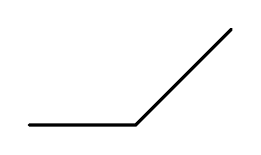
\begin{tikzpicture}[scale=0.9, line cap=round]
  \axes
  \draw[very thick] (-1.5,0)--(0,0)--(1.35,1.35);
\end{tikzpicture}\\[2pt]
(b) ReLU
\end{minipage}\hfill
%
\begin{minipage}[t]{0.31\linewidth}\centering

\begin{tikzpicture}[scale=0.9, line cap=round]
  \axes
  \draw[very thick] (-1.4,-0.8)--(1.4,1.3);
\end{tikzpicture}\\[2pt]
(c) Linear
\end{minipage}
\end{center}

\vspace{4pt}
{\small (i) Which curve --- (a), (b), or (c) --- belongs on that final neuron, and why?}\\[2pt]
\hspace*{1.5em}\rb{(a) Sigmoid --- its output is squeezed into $(0,1)$, so it reads as a probability}{10.5cm}\\[6pt]
{\small (ii) A hidden \textbf{ReLU} neuron receives weighted sum $z=-3$. Its output $=$}\;\; \rb{$0$}{1.6cm}\\[6pt]
{\small (iii) The final \textbf{sigmoid} neuron receives $z=0$. The probability it reports $\approx$}\;\; \rb{$0.5$}{1.6cm}

\keybox{(i) Curve \textbf{(a), the sigmoid} --- it is the only activation whose output is bounded
to $(0,1)$, so it can be read as a probability; ReLU is unbounded above and the linear line is
unbounded both ways, so neither can report a probability. (ii) $\operatorname{ReLU}(-3)=\max(0,-3)=0$
--- the neuron is silent. (iii) $\operatorname{sigmoid}(0)=1/(1+e^{0})=1/2=0.5$ --- maximally
uncertain, a coin flip.}

\vspace{2pt}\hrule\vspace{5pt}

% =========================== Q2 ===========================
\textbf{2. One neuron, by hand.}\; {\small Compute the weighted sum $z$, then pass it through
ReLU.}

\vspace{2pt}
\textbf{Given:}\quad $x_1 = 2,\ \ x_2 = 3 \qquad w_1 = 0.5,\ \ w_2 = -1 \qquad b = 1$

\[
z = w_1 x_1 + w_2 x_2 + b = \blk{5.5cm} = \rb{$-1$}{1.3cm}
\]
\[
\text{output} = \operatorname{ReLU}(z) = \max(0,\,z) = \rb{$0$}{1.3cm}
\]

\work{0.9cm}

\keybox{$z = (0.5)(2) + (-1)(3) + 1 = 1 - 3 + 1 = -1$, so
$\operatorname{ReLU}(-1) = \max(0,-1) = 0$. ReLU clips the negative sum to zero: for this
input the neuron stays silent.}

\vspace{2pt}\hrule\vspace{5pt}

% =========================== Q3 ===========================
\textbf{3. A whole layer in one step.}\; {\small Multiply the $2\times3$ weight matrix by the
input vector.}

\[
\mathbf{W}\mathbf{x} =
\underbrace{\begin{pmatrix} 1 & 0 & 2 \\ -1 & 3 & 1 \end{pmatrix}}_{\mathbf{W}}
\underbrace{\begin{pmatrix} 2 \\ 1 \\ 0 \end{pmatrix}}_{\mathbf{x}}
= \begin{pmatrix} \blk{3.4cm} \\[3pt] \blk{3.4cm} \end{pmatrix}
= \begin{pmatrix} \rb{$2$}{1cm} \\[3pt] \rb{$1$}{1cm} \end{pmatrix}
\]

\work{0.7cm}

\keybox{Row 1: $(1)(2)+(0)(1)+(2)(0) = 2$. \ Row 2: $(-1)(2)+(3)(1)+(1)(0) = 1$. \ Hence
$\mathbf{W}\mathbf{x} = \left(\begin{smallmatrix}2\\1\end{smallmatrix}\right)$. A $2\times3$
matrix times a length-$3$ vector yields a length-$2$ output --- one number per neuron: a full
forward pass.}

\vspace{2pt}\hrule\vspace{5pt}

% =========================== Q4 ===========================
\textbf{4. Learned or engineered?}\; {\small Two ways to call \emph{resistant} vs.\
\emph{susceptible} from a MALDI-TOF spectrum:}

\vspace{2pt}
\textbf{Pipeline A} --- a technician computes the peak area at $m/z\ 2415$ and the $2415/4100$
ratio, then feeds those two numbers to logistic regression.

\textbf{Pipeline B} --- the raw $6{,}000$-bin spectrum goes straight into a neural network,
which forms its own internal ``peak-ish here'' detector in an early layer.

\vspace{3pt}
Which pipeline uses \emph{hand-engineered} features, and which uses \emph{learned} features?

\vspace{3pt}
hand-engineered $\rightarrow$ Pipeline \rb{A}{1.6cm}
\hfill
learned $\rightarrow$ Pipeline \rb{B}{1.6cm}
\hspace*{2cm}

\keybox{Hand-engineered $\rightarrow$ A; learned $\rightarrow$ B. In A a human chose the peak
area and the ratio (hand-engineered features); in B the network discovers its own ``peak-ish''
detector directly from the raw spectrum (learned features). That shift is the essence of deep
learning.}

\vspace{2pt}\hrule\vspace{5pt}

% =========================== Q5 ===========================
\textbf{5. In one sentence.}\; {\small What is the core difference between deep learning and
classic machine learning?}

\work{1.4cm}
\ifsolution\else\blk{\linewidth}\\[10pt]\blk{\linewidth}\fi

\keybox{Deep learning learns its own features straight from raw data, whereas classic machine
learning relies on features a human engineers first. (Any answer capturing ``learned features
from raw data'' vs.\ ``human-engineered features'' earns full credit; phrasing about
representation learning or end-to-end training is equally acceptable.)}

\vspace{2pt}\hrule\vspace{5pt}

% =========================== Q6 ===========================
\textbf{6. Two layers, by hand.}\; {\small Run a full two-layer forward pass: first the
hidden layer (matrix--vector, add bias, then ReLU), then the output layer.}

\vspace{2pt}
\textbf{Layer 1:}\quad
$\mathbf{W_1} = \begin{pmatrix} 1 & -1 \\ -1 & 1 \end{pmatrix},\quad
\mathbf{x} = \begin{pmatrix} 2 \\ 1 \end{pmatrix},\quad
\mathbf{b_1} = \begin{pmatrix} 0 \\ -4 \end{pmatrix}$

\[
\mathbf{h} = \operatorname{ReLU}(\mathbf{W_1}\mathbf{x} + \mathbf{b_1})
= \operatorname{ReLU}\!\begin{pmatrix} \blk{2.2cm} \\[3pt] \blk{2.2cm} \end{pmatrix}
= \begin{pmatrix} \rb{$1$}{1cm} \\[3pt] \rb{$0$}{1cm} \end{pmatrix}
\]

\textbf{Layer 2:}\quad
$\mathbf{W_2} = \begin{pmatrix} 3 & 2 \end{pmatrix},\quad b_2 = -1$

\[
y = \mathbf{W_2}\mathbf{h} + b_2 = \blk{5cm} = \rb{$2$}{1.3cm}
\]

\work{0.9cm}

\keybox{Layer 1: row 1 $=(1)(2)+(-1)(1)+0 = 1$, so $\operatorname{ReLU}(1)=1$; row 2
$=(-1)(2)+(1)(1)+(-4) = -5$, so $\operatorname{ReLU}(-5)=0$. Hence
$\mathbf{h} = \left(\begin{smallmatrix}1\\0\end{smallmatrix}\right)$ --- the second hidden
neuron stays silent. Layer 2: $y = (3)(1)+(2)(0)-1 = 2$. The input $(2,1)$ here is the
layer output $\mathbf{Wx}$ from Q3 carried forward --- a layer's output is simply the
next layer's input, and stacking that same move is what ``deep'' means.}

\vspace{4pt}\hrule\vspace{3pt}
{\small\itshape \ifsolution Answer key.\else Keep this sheet --- the neuron and matrix drills
are your Lab 1 cheat-sheet.\fi}

\end{document}
"
%  (or, to flip by hand, change \solutionfalse to \solutiontrue below.)
% =====================================================================
\documentclass[11pt]{article}

\newif\ifsolution
\ifdefined\showsolutions \solutiontrue \else \solutionfalse \fi
% \solutiontrue   % <-- uncomment to hard-code the ANSWER KEY build

\usepackage[letterpaper, margin=0.6in, top=0.7in, bottom=0.5in]{geometry}
\usepackage{amsmath, amssymb}
\usepackage{xcolor}
\usepackage{tikz}
\usepackage{fancyhdr}

\pagestyle{fancy}
\fancyhf{}
\fancyhead[L]{\small\textbf{MSACL DS301 --- Deep Learning}}
\fancyhead[R]{\small\textbf{Quiz 1: Foundations\ifsolution\ \textmd{(Answer Key)}\fi}}
\fancyfoot[C]{\thepage}
\renewcommand{\headrulewidth}{0.4pt}

\newcommand{\blk}[1]{\underline{\hspace{#1}}}
% Reveal-or-blank: shows the answer in the key, a blank rule on the student sheet.
\newcommand{\rb}[2]{\ifsolution\textbf{#1}\else\blk{#2}\fi}
% Boxed answer (key only) and blank writing space (student only).
\newcommand{\keybox}[1]{\ifsolution\par\vspace{2pt}%
  \fbox{\parbox{0.965\textwidth}{\small\textbf{Answer.}\; #1}}\par\fi}
\newcommand{\work}[1]{\ifsolution\else\vspace{#1}\fi}

\setlength{\parindent}{0pt}
\setlength{\parskip}{3pt}
\setlength{\abovedisplayskip}{5pt}
\setlength{\belowdisplayskip}{5pt}

\begin{document}

\begin{center}
{\Large \textbf{Quiz 1 --- Foundations}}\\[2pt]
{\normalsize The neuron, activation functions, a layer as a matrix, and a two-layer pass}
\end{center}

\vspace{-2pt}
\begin{center}
\fbox{\parbox{0.92\textwidth}{\small
\textbf{Instructions:}\; Answer all six questions. Intuition first, light arithmetic ---
show your work on the blanks. No calculators needed.%
\ifsolution\else\\[4pt]\textbf{Name:}\ \blk{6cm}\hfill\textbf{Date:}\ \blk{3.5cm}\fi
}}
\end{center}

\vspace{-2pt}\hrule\vspace{5pt}

% =========================== Q1 ===========================
\textbf{1. Pick the activation, then compute.}\; {\small Your MRSA classifier's \emph{final} neuron
must output a probability between $0$ and $1$ that the isolate is \emph{resistant}. The three
activation shapes are below.}

\vspace{3pt}
\begin{center}
\newcommand{\axes}{\draw[->,gray] (-1.6,0)--(1.95,0); \draw[->,gray] (0,-0.9)--(0,1.6);}
%
\begin{minipage}[t]{0.31\linewidth}\centering

\begin{tikzpicture}[scale=0.9, line cap=round]
  \axes
  \draw[very thick, samples=80, domain=-1.5:1.85] plot (\x,{1.2/(1+exp(-4*\x))});
\end{tikzpicture}\\[2pt]
(a) Sigmoid
\end{minipage}\hfill
%
\begin{minipage}[t]{0.31\linewidth}\centering
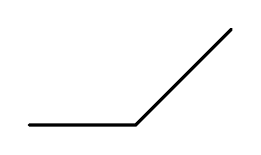
\begin{tikzpicture}[scale=0.9, line cap=round]
  \axes
  \draw[very thick] (-1.5,0)--(0,0)--(1.35,1.35);
\end{tikzpicture}\\[2pt]
(b) ReLU
\end{minipage}\hfill
%
\begin{minipage}[t]{0.31\linewidth}\centering

\begin{tikzpicture}[scale=0.9, line cap=round]
  \axes
  \draw[very thick] (-1.4,-0.8)--(1.4,1.3);
\end{tikzpicture}\\[2pt]
(c) Linear
\end{minipage}
\end{center}

\vspace{4pt}
{\small (i) Which curve --- (a), (b), or (c) --- belongs on that final neuron, and why?}\\[2pt]
\hspace*{1.5em}\rb{(a) Sigmoid --- its output is squeezed into $(0,1)$, so it reads as a probability}{10.5cm}\\[6pt]
{\small (ii) A hidden \textbf{ReLU} neuron receives weighted sum $z=-3$. Its output $=$}\;\; \rb{$0$}{1.6cm}\\[6pt]
{\small (iii) The final \textbf{sigmoid} neuron receives $z=0$. The probability it reports $\approx$}\;\; \rb{$0.5$}{1.6cm}

\keybox{(i) Curve \textbf{(a), the sigmoid} --- it is the only activation whose output is bounded
to $(0,1)$, so it can be read as a probability; ReLU is unbounded above and the linear line is
unbounded both ways, so neither can report a probability. (ii) $\operatorname{ReLU}(-3)=\max(0,-3)=0$
--- the neuron is silent. (iii) $\operatorname{sigmoid}(0)=1/(1+e^{0})=1/2=0.5$ --- maximally
uncertain, a coin flip.}

\vspace{2pt}\hrule\vspace{5pt}

% =========================== Q2 ===========================
\textbf{2. One neuron, by hand.}\; {\small Compute the weighted sum $z$, then pass it through
ReLU.}

\vspace{2pt}
\textbf{Given:}\quad $x_1 = 2,\ \ x_2 = 3 \qquad w_1 = 0.5,\ \ w_2 = -1 \qquad b = 1$

\[
z = w_1 x_1 + w_2 x_2 + b = \blk{5.5cm} = \rb{$-1$}{1.3cm}
\]
\[
\text{output} = \operatorname{ReLU}(z) = \max(0,\,z) = \rb{$0$}{1.3cm}
\]

\work{0.9cm}

\keybox{$z = (0.5)(2) + (-1)(3) + 1 = 1 - 3 + 1 = -1$, so
$\operatorname{ReLU}(-1) = \max(0,-1) = 0$. ReLU clips the negative sum to zero: for this
input the neuron stays silent.}

\vspace{2pt}\hrule\vspace{5pt}

% =========================== Q3 ===========================
\textbf{3. A whole layer in one step.}\; {\small Multiply the $2\times3$ weight matrix by the
input vector.}

\[
\mathbf{W}\mathbf{x} =
\underbrace{\begin{pmatrix} 1 & 0 & 2 \\ -1 & 3 & 1 \end{pmatrix}}_{\mathbf{W}}
\underbrace{\begin{pmatrix} 2 \\ 1 \\ 0 \end{pmatrix}}_{\mathbf{x}}
= \begin{pmatrix} \blk{3.4cm} \\[3pt] \blk{3.4cm} \end{pmatrix}
= \begin{pmatrix} \rb{$2$}{1cm} \\[3pt] \rb{$1$}{1cm} \end{pmatrix}
\]

\work{0.7cm}

\keybox{Row 1: $(1)(2)+(0)(1)+(2)(0) = 2$. \ Row 2: $(-1)(2)+(3)(1)+(1)(0) = 1$. \ Hence
$\mathbf{W}\mathbf{x} = \left(\begin{smallmatrix}2\\1\end{smallmatrix}\right)$. A $2\times3$
matrix times a length-$3$ vector yields a length-$2$ output --- one number per neuron: a full
forward pass.}

\vspace{2pt}\hrule\vspace{5pt}

% =========================== Q4 ===========================
\textbf{4. Learned or engineered?}\; {\small Two ways to call \emph{resistant} vs.\
\emph{susceptible} from a MALDI-TOF spectrum:}

\vspace{2pt}
\textbf{Pipeline A} --- a technician computes the peak area at $m/z\ 2415$ and the $2415/4100$
ratio, then feeds those two numbers to logistic regression.

\textbf{Pipeline B} --- the raw $6{,}000$-bin spectrum goes straight into a neural network,
which forms its own internal ``peak-ish here'' detector in an early layer.

\vspace{3pt}
Which pipeline uses \emph{hand-engineered} features, and which uses \emph{learned} features?

\vspace{3pt}
hand-engineered $\rightarrow$ Pipeline \rb{A}{1.6cm}
\hfill
learned $\rightarrow$ Pipeline \rb{B}{1.6cm}
\hspace*{2cm}

\keybox{Hand-engineered $\rightarrow$ A; learned $\rightarrow$ B. In A a human chose the peak
area and the ratio (hand-engineered features); in B the network discovers its own ``peak-ish''
detector directly from the raw spectrum (learned features). That shift is the essence of deep
learning.}

\vspace{2pt}\hrule\vspace{5pt}

% =========================== Q5 ===========================
\textbf{5. In one sentence.}\; {\small What is the core difference between deep learning and
classic machine learning?}

\work{1.4cm}
\ifsolution\else\blk{\linewidth}\\[10pt]\blk{\linewidth}\fi

\keybox{Deep learning learns its own features straight from raw data, whereas classic machine
learning relies on features a human engineers first. (Any answer capturing ``learned features
from raw data'' vs.\ ``human-engineered features'' earns full credit; phrasing about
representation learning or end-to-end training is equally acceptable.)}

\vspace{2pt}\hrule\vspace{5pt}

% =========================== Q6 ===========================
\textbf{6. Two layers, by hand.}\; {\small Run a full two-layer forward pass: first the
hidden layer (matrix--vector, add bias, then ReLU), then the output layer.}

\vspace{2pt}
\textbf{Layer 1:}\quad
$\mathbf{W_1} = \begin{pmatrix} 1 & -1 \\ -1 & 1 \end{pmatrix},\quad
\mathbf{x} = \begin{pmatrix} 2 \\ 1 \end{pmatrix},\quad
\mathbf{b_1} = \begin{pmatrix} 0 \\ -4 \end{pmatrix}$

\[
\mathbf{h} = \operatorname{ReLU}(\mathbf{W_1}\mathbf{x} + \mathbf{b_1})
= \operatorname{ReLU}\!\begin{pmatrix} \blk{2.2cm} \\[3pt] \blk{2.2cm} \end{pmatrix}
= \begin{pmatrix} \rb{$1$}{1cm} \\[3pt] \rb{$0$}{1cm} \end{pmatrix}
\]

\textbf{Layer 2:}\quad
$\mathbf{W_2} = \begin{pmatrix} 3 & 2 \end{pmatrix},\quad b_2 = -1$

\[
y = \mathbf{W_2}\mathbf{h} + b_2 = \blk{5cm} = \rb{$2$}{1.3cm}
\]

\work{0.9cm}

\keybox{Layer 1: row 1 $=(1)(2)+(-1)(1)+0 = 1$, so $\operatorname{ReLU}(1)=1$; row 2
$=(-1)(2)+(1)(1)+(-4) = -5$, so $\operatorname{ReLU}(-5)=0$. Hence
$\mathbf{h} = \left(\begin{smallmatrix}1\\0\end{smallmatrix}\right)$ --- the second hidden
neuron stays silent. Layer 2: $y = (3)(1)+(2)(0)-1 = 2$. The input $(2,1)$ here is the
layer output $\mathbf{Wx}$ from Q3 carried forward --- a layer's output is simply the
next layer's input, and stacking that same move is what ``deep'' means.}

\vspace{4pt}\hrule\vspace{3pt}
{\small\itshape \ifsolution Answer key.\else Keep this sheet --- the neuron and matrix drills
are your Lab 1 cheat-sheet.\fi}

\end{document}
